The third test activity, which involved important research for the \gls{STS} is related to the designing and testing of different relative humidity and temperature sensors. Due to the harsh conditions in the detector, choosing humidity sensors is an important task that should ensure the operational safety of the detector. This chapter presents the overview of different solutions for ambient sensing, together with answers to whether the tested technology meets the requirements. Most efforts were made to characterize fiber optic sensors, and subsequently come up with safety requirements and system that would address potential risks posed by e.g., too humid environment. 

%% Add here some more text about the used DCS framework

\section{Sensors requirements}

The design of the \gls{STS} \cite{Heuser:54798} defines the requirements for potential ambient sensors. As described in the section~\ref{STS}, the ambient temperature will reach \SI{-10}{\celsius} at the end of the \gls{STS}'s lifetime. The cooling liquid (3M NOVEC 649) will be circulating at temperatures close to~\SI{-40}{\celsius}. Therefore, the first boundary condition arises: the frost point and dew point inside the \gls{STS} has to be below~\SI{-40}{\celsius} to avoid ice formation or condensation on the \gls{FEE}.
During the first few years of operation, the temperatures will be higher and Relative Humidity (\gls{RH}) can be measured more accurately\footnote{performance of the commercial RH sensors usually decreases below \SI{0}{\degree}}. 
%One of the most common techniques to achieve the frost points below~\SI{-40}{\celsius} is baking. In the case of the silicon tracker, too high temperatures could destroy the~\gls{FEE}. 

During the detector's lifetime (10 years), there will be few opportunities to perform any upgrades. Therefore, the sensors have to withstand the radiation accumulated during that period (about 10kGy). As few sensors will be placed in the vicinity of the beam pipe, the total dose could reach more than 10\,kGy~\cite{Heuser:54798}. The humidity measurements will be distributed, implying that different sensors may face different doses. 
The humidity sensors have to be insensitive to the magnetic field of \SI{1}{\tesla\metre} since the whole detector resides in a dipole magnet.  An ideal humidity sensor should also meet the following requirements:
\begin{itemize}
    \item small dimensions and mass (especially when placed close to the active area of the system),
    \item accurate relative humidity readouts at temperatures down to~\SI{-20}{\celsius}, 
    \item respond to a wide range of \gls{RH} values from 0\% to 80\%,
    \item high repeatability and low hysteresis,
    \item reliable operation across long distances (the readout device will be at least~\SI{20}{\metre} away from the detector).
\end{itemize}

On the other hand, due to overpressure conditions inside the \gls{STS} enclosure, a low response time (seconds) is not necessarily needed. In terms of detector safety and implementation of the sensors readouts in the hardware and software interlocking, the time response up to minutes is considered to be acceptable. 

\section{Vapor pressure and its significance}

The \gls{RH}, or the dew/frost point, are commonly used indicators to describe the number of water molecules in the air. The temperature at which water vapor in any gas medium (at constant pressure) begins to condense into liquid water at the same rate at which it evaporates, which is a measure of how much water vapor is in a gas medium, is known as the dew point.

Water vapor condenses as liquid water at gas temperatures above \SI{0}{\celsius}. The dew point is defined as a liquid condensation layer. Water vapor condenses as solid ice at gas temperatures far below \SI{0}{\celsius}. The frost point is defined as a solid condensation layer. However, for gas temperatures ranging from \SI{0}{\celsius} to approximately \SI{-20}{\celsius}, the state of the condensed layer is unknown; it could be either water, ice, or a combination of both \cite{nie_dewpoint}. 


The first documented formula for vapor pressure (over water and over ice) was introduced by Goff and Gratch in 1945 \cite{goff_gratch}. The original correlation (over water) is as follows:

\begin{equation}
\label{gratch}
\begin{split}
    &log({e}^{*}_{s}) = a(T_{st}/T - 1) + b(log(T_{st}/T) - c(10^{11.344(1-T/T_{st})} - 1) \\
    &+ d(10^{-3.49149(T_{st}/T - 1} -1) + log(e^{*}_{st})
\end{split}
\end{equation}
where log refers to the logarithm base 10, $e_{s}$ is the saturation water vapor pressure~(hPa), a to d are constants; $a = - 7.90$, $b=5.03$, $c=1.38\times10^{-7}$, $d=1.38\times10^{-7}$, $e^{*}_{s}$ is the stream-point pressure ($1013.246\,hPa$), and $T_{st}$ is the boiling point (at 1\,atm) temperature (373.15\,K). A similar equation can also be formulated for the vapor pressure over ice. 

These equations marked the first attempts to formulate a highly accurate description of water dynamics in the air. The Magnus formula is easier to implement than Equation~\ref{gratch} and allows converting between the saturation vapor pressure and temperature with a minimal error~\cite{magnus}: 
\begin{equation}
    e^{*}_{s} = c*e^{(aT/(b+T))}
\end{equation}
where \gls{RH} is usually defined as the ratio of the water vapor pressure ($e$) to the equilibrium vapor pressure over water plane ($e^{*}_{s}$):
\begin{equation}
    RH = 100\frac{e}{e^{*}_{s}}
    \label{eq:RH}
\end{equation}
Based on the parameters approximations by Sonntag ($c=6.11$\,hPa, $a=17.62$, $b=243.12$\,\SI{}{\celsius}) \cite{magnus}, the formula converges to:
\begin{equation}
    e^{*}_{s} = 6.112*e^{(17.62T/(243.12))}
    \label{eq:pressure}
\end{equation}
The dew formation corresponds to the equation:
\begin{equation}
    e^{*}_{s}(T_{d}) = e_{st}(T)
    \label{eq:dew}
\end{equation}
Sonntag approximation provides a maximum error of \SI{0.35}{\celsius} between \SI{-45}{\celsius} and \SI{60}{\celsius} in comparison to the more complex formula described in \cite{hardy}. 
Inserting the equation \ref{eq:RH} and \ref{eq:pressure} to the \ref{eq:dew} leads to the formula below, which provides the dew point in \SI{}{\celsius}.
\begin{equation}
    T_{d}(T, RH) = \frac{\lambda(ln(\frac{RH}{100})+\frac{\beta T}{\lambda + T})}{\beta - (ln(\frac{RH}{100})+\frac{\beta T}{\lambda + T}}
    \label{eq:td}
\end{equation}
\begin{figure}[!h]
\centering
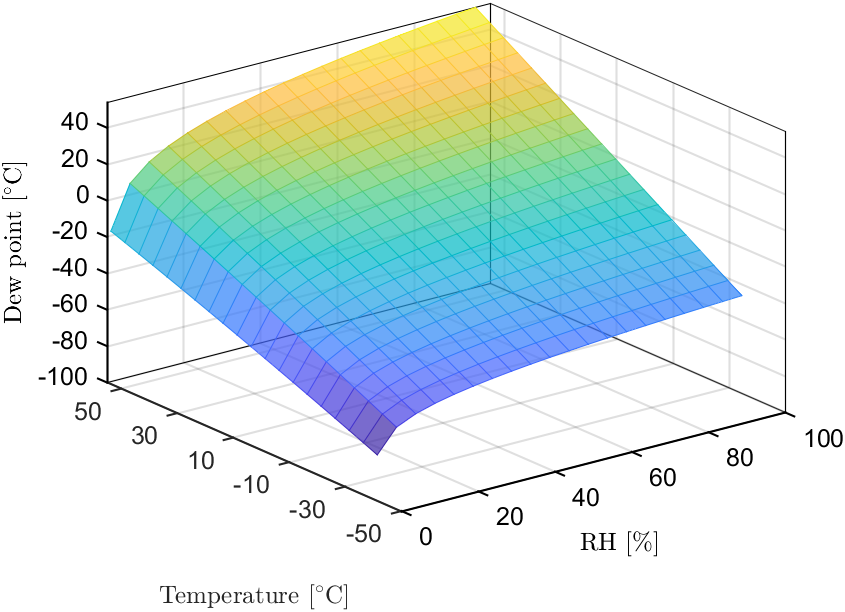
\includegraphics[width=0.65\columnwidth]{Chapter5/images/dewpointmagnus.png}
\caption{Dew points calculations based on the Magnus formula with parameters approximations by Sonntag.}
\label{fig:dewpointmagnus}
\end{figure}

The dew points based on relative humidity and temperature can be seen in Figure~\ref{fig:dewpointmagnus}. In order to compare the results of different relative humidity sensors and dew points sensors, uncertainties of the dry-bulb\footnote{"Dry Bulb Temperature" refers essentially to the ambient air temperature. It is called "Dry Bulb" because the air temperature is indicated by a thermometer, not affected by the moisture of the air.} temperature and \gls{RH} are required.

The individual standard uncertainty $\mu$ is defined as the uncertainty of the result of a measurement expressed as its standard deviation~\cite{NIST_1994}. Hence, assuming the rectangular\footnote{constant in the defined range} distribution of uncertainty for the sensors that measure the temperature and relative humidity:
\begin{equation}
    \mu(x_{i}) = \frac{a}{\sqrt{3}}
\end{equation}
where a is the uncertainty available in the datasheets, and $x_{i}$ represents the measured value. The combined uncertainty $\mu_{c}$ can be derived from Equation \ref{eq:dew} based on the law of propagation of uncertainty~\cite{dp_uncertainty}:
\begin{equation}
    u_{Td} = \left [  \left (\frac{\partial T_{d}}{\partial T_{a}}  \right )^{2} \mu^{2}(T) + \left (\frac{\partial T_{d}}{\partial RH}  \right )^{2} \mu^{2}(RH)\right ]^{1/2}
    \label{dp_error}
\end{equation}

In each system, we assume that measuring dew point temperature or relative humidity is statistically independent of measuring air temperature and the confidence level for the uncertainty interval is 68\%.  
%Moreover, below~\SI{0}{\celsius} the frost point starts to play a key role. The moisture in the air will undergo deposition as a layer of frost on exposed surfaces that are also at a temperature below the frost point. 

\section{Overview of different technologies}

Nowadays, electronic humidity sensors are commonly used in industry, scientific research facilities, and civil infrastructure. In general, we can classify the sensors based on their operating principle - changes in current, voltage, weight, or conductivity can be subsequently associated with humidity changes if the underlying detection principles relate to interaction with water. Resistive and capacitive sensors represent over 75\% of all the sensors used today. As the names indicate, their working principles are based on resistance and capacitance changes, respectively.


The efforts to employ miniaturized sensors in the \gls{HEP} experiment have been ongoing for many years. A general review of the dew point and relative humidity sensing techniques was presented in~\cite{RITTERSMA}. On the other hand, a more recent overview with a case-specific study related to \gls{HEP} is summarized in~\cite{Kapic}.

The two most challenging requirements in the case of \gls{STS} are radiation hardness and insensitivity to the magnetic field. Radiation can affect sensor materials in different ways depending on their type, rate of interaction, and material composition. Sensor structures are affected by radiation due to modifications to their lattice structures. For example, capacitive sensors like HIH3610~\cite{HIH3610} and HIH4030~\cite{HIH4030} tested in CERN turned out to be critically damaged after irradiation~\cite{Berruti}. It was also recently reported that capacitive sensors from IST AG~\cite{MK33} has a linear response to the radiation (what can be corrected~\cite{Kapic_sensor}). Employing such sensors in a \gls{HEP} experiment, especially in a tracker surrounded by a magnet, raises questions about the sensitivity to the magnetic field~\cite{Berruti}. 

One of the possible solutions is using fiber optic-based sensors, which are by design not insensitive to the magnetic field. Another possibility is to use a sampling system, which sucks the air from the detector and using e.g., a vacuum pump transports it to the area with lower radiation and without a magnetic field.

For the \gls{STS} a distributed sensing system featuring a few different technologies is considered. The following sensors are discussed in the next sections: capacitive, fiber optic, and dew point transmitters. 


\subsection{Industrial capacitive sensors and their performance at negative temperatures}
\label{capacitive_sensors}
The capacitive sensors, in the simplest form, can be made out of two parallel plates, where the capacitance between the two electrodes is given by:
\begin{equation}
C = \epsilon_{r}\epsilon_0\frac{A}{d}
\end{equation}
where the $\epsilon_{r}$ and $\epsilon_{0}$ are the relative and vacuum permittivity constants, A is the plate surface area and d is the plate distance. If the humidity changes can be associated with the changes of one of the parameters, the \gls{RH} can be therefore calculated. 
The capacitive \gls{RH} sensors can measure below \SI{0}{\celsius}, they are fairly miniaturized and insensitive to pressure changes. The main drawbacks of these sensors are listed below:
\begin{itemize}
    \item limited long-term stability,
    \item sensitive to water condensation,
    \item limited distance to the readout device,
    \item most of the sensors are not radiation-hard.
\end{itemize}
Two different \gls{RH} capacitive sensors have been tested in low-temperature regimes - IST HYT221~\cite{hyt221} and Sensiron SHT85~\cite{SHT85}. Figure \ref{fig:hyt221} depicts the \gls{RH} and temperature accuracy. Measuring humidity at low temperatures below \SI{-20}{\celsius} and 5\% \gls{RH} leads to large dew point errors (\SI{7}{\celsius} and more). The estimated dew point errors are presented in figure \ref{fig:hyt221_dp}.
\begin{figure}[!h]
\centering
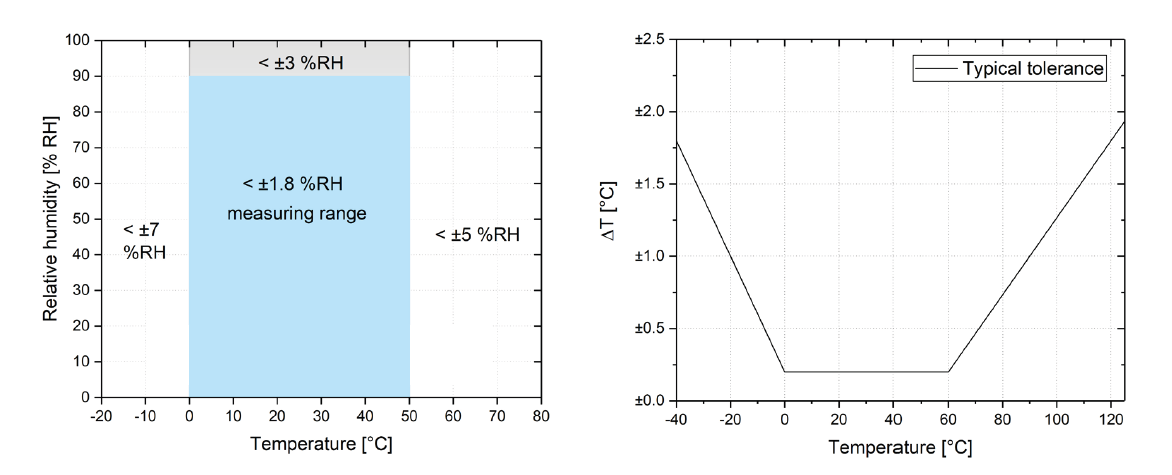
\includegraphics[width=0.9\columnwidth]{Chapter5/images/hyt221_rh.png}
\caption{Relative humidity and temperature uncertainties of the IST AG HYT221 sensor in different environmental conditions~\cite{hyt221}.}
\label{fig:hyt221}
\end{figure}
\begin{figure}[!h]
\centering
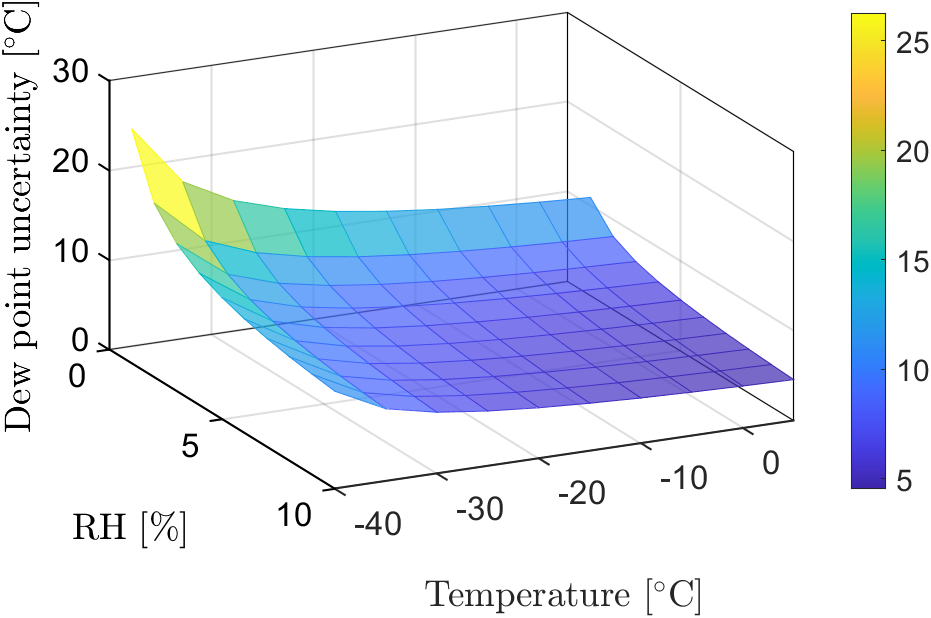
\includegraphics[width=0.6\columnwidth]{Chapter5/images/HYT221RH7T15.png}
\caption{Dew point error based on values from Figure \ref{fig:hyt221} for IST AG HYT221.}
\label{fig:hyt221_dp}
\end{figure}
\newpage
Figure \ref{fig:sht85} shows the uncertainties for the measurements with the SHT85 sensor above \SI{0}{\celsius}. The data below \SI{0}{\celsius} is not provided, therefore an extrapolation was made in order to have a comparison with the HYT221 sensor. The results are presented in Figure~\ref{fig:sht85_dp}. In this case, the errors reach up to \SI{5}{\celsius} in the lowest temperatures and \gls{RH} levels.
\begin{figure}[!h]
\centering
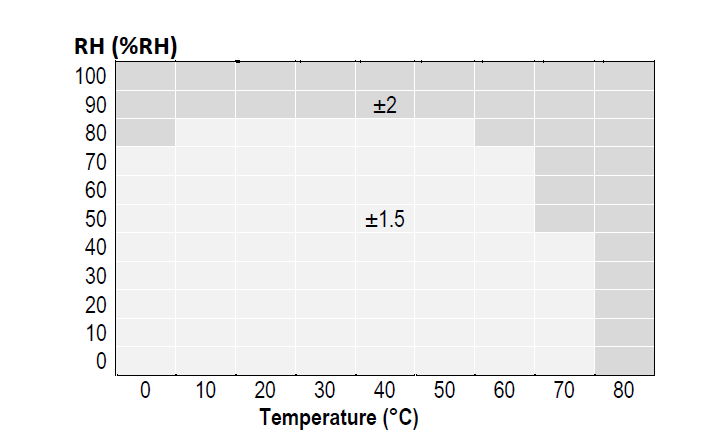
\includegraphics[width=0.65\columnwidth]{Chapter5/images/sht85_rh.png}
\caption{Relative humidity uncertainties for the SHT85 hygrometer, the temperature uncertainty is \SI{0.2}{\celsius} \cite{SHT85}.}
\label{fig:sht85}
\end{figure}

\begin{figure}[!h]
\centering
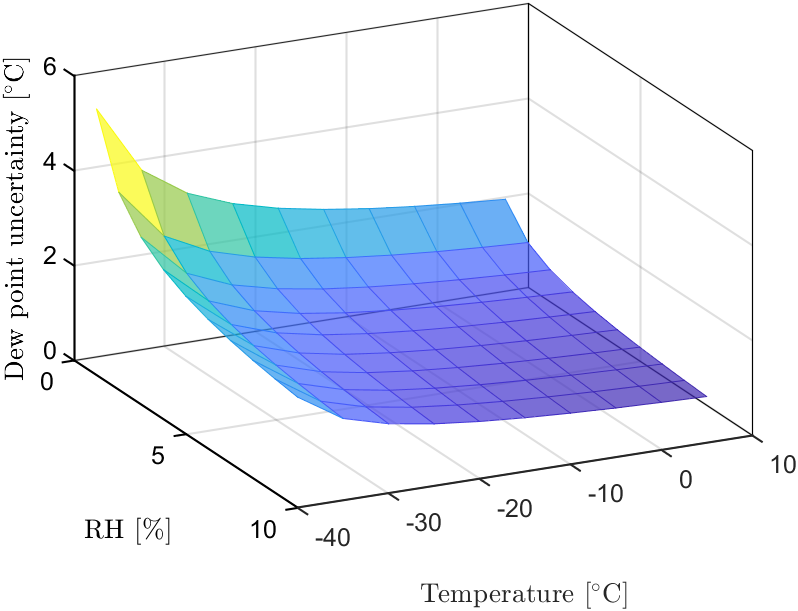
\includegraphics[width=0.6\columnwidth]{Chapter5/images/SHTRH15T02.png}
\caption{Dew point error based on Figure \ref{fig:sht85}.}
\label{fig:sht85_dp}
\end{figure}
\newpage
The above-presented results don't take into account additional effects that alter the calculations, like hysteresis or drift, which could together contribute by 1\% or more to the \gls{RH} measurement. The performance of the SHT85 also decreases in the low-temperature regime, but the extent is not determined in this work. The comparison of the industrial capacitive sensors shows a large performance disproportion.

The studied sensors are much cheaper than custom trace humidity measurement systems (sampling systems) or fiber optic sensors. The readout of such sensors may be affected by the radiation and magnetic field, so they can't be considered a reliable solution for a long-term operation in the \gls{STS}. The next type of sensor that yields promising results is based fiber optic sensing technology~\ref{FOS}.

\subsection{Description of the Fiber Optic Sensing technology}
\label{FOS}

Fiber optic sensors-based (\gls{FOS}) system usually consists of three main components as optical source, transducer, and detector. In general, the sensing principle relies on modifying one or more properties of light (most commonly a laser, diodes, or LEDs are employed as the optical sources) passing through a transducer which is located inside the fiber. A schematic view of a sensing setup is presented in Figure~\ref{fig:sensing}. Distributed sensing or even continuous sensing offers a unique opportunity for many sensing points in one fiber~\cite{GRATTAN200040}. 
\newpage
\begin{figure}[!h]
\centering
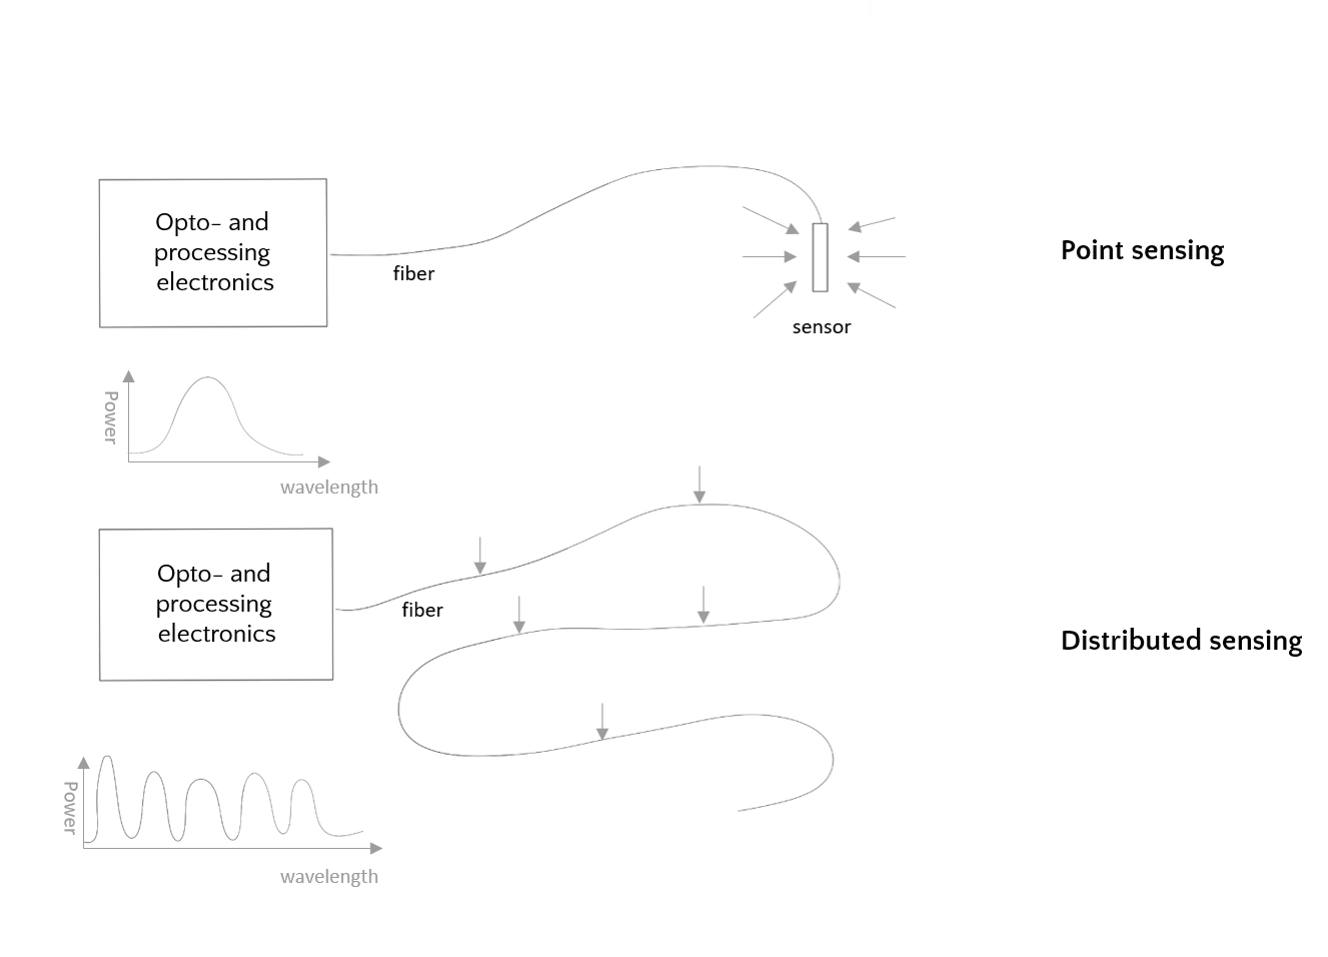
\includegraphics[width=0.95\columnwidth]{Chapter5/images/sensing.png}
\caption{Comparison of different sensing possibilities with the \gls{FOS}. Opto- and processing electronics is commonly called optical interrogator.}
\label{fig:sensing}
\end{figure}

In general, humidity sensing can be classified according to the underlying operating principles~\cite{fos_overview}. Furthermore, we can distinguish intrinsic and extrinsic sensors that indicate whether sensing occurs inside or outside the fiber. The main effort has focused on in-fiber grating sensors, which belong to a class of intrinsic \gls{FOS} that has gained popularity in recent years. 

The main efforts were concentrated on a technology called Fiber Bragg Grating. The driving factor for this decision was the successful implementation of the sensors of this type in the Compact Muon Solenoid (\gls{CMS}) at \gls{CERN}, which was extensively reported in a number of papers and summarized in~\cite{Berruti}. Moreover, a few similar implementations were summarized in~\cite{YEO_PI} and ~\cite{Kronenberg:02}. 

Fiber optic sensors have notable advantages in comparison to conventional sensors:

\begin{itemize}
    \item fibers can be insensitive to radiation or have predictable behavior,
    \item magnetic field insensitive,
    \item good signal transmission over long distances,
    \item multiplexing capabilities (see figure~\ref{fig:sensing}),
    \item immunity to electrostatic and electromagnetic interference,
    \item resistant to harsh conditions - the sensors are completely passive elements, hence they offer long durability.
\end{itemize}

On the other hand, \gls{FOS} are difficult to integrate with hardware interlocks, handling, and installation of the sensors might be more challenging due to the risk of damaging the fiber.




\subsubsection{Fiber Bragg Grating based sensor for humidity monitoring }
\label{fbg}
A Fiber Bragg Grating (\glspl{FBG}) is a selective filter inside the optical fiber that reflects light signals at a specific wavelength known as the Bragg wavelength ($\lambda_{B}$). Such a filter is created by inscribing a systematic variation of the fiber's refractive index~\cite{fbg_overview}. This characteristic wavelength ($\lambda_{B}$) is dependent on the fiber effective refractive index ($\eta_{eff}$) and the grating pitch ($\Lambda$) of the \gls{FBG}~\cite{Othonos2000FiberBG}:
\begin{equation}
    \lambda_{B} = 2 \eta_{eff} \Lambda
\end{equation}

Both factors can be affected by strain, temperature, magnetic field, and/or pressure changes, thus various sensing possibilities are available with the ~\cite{Yun-Jiang_Rao_1997}. In general, wavelength shift $\lambda_{B}$ can be formulated as:

\begin{equation}
    \frac{\Delta\lambda_{B}}{\lambda_{B}}=(1-P_{e}) \epsilon + \left [(1-P_{e}) \alpha + \xi  \right ] \Delta T
\end{equation}

where $P_{e}$ is a photo-elastic constant (optical properties change under mechanical deformation), $\epsilon$ is a strain induced on the fiber, $\alpha$ is the thermal expansion coefficient of the coated \gls{FBG}, and the $\xi$ is the thermo-optic coefficient (change of the refractive index with the temperature) of the fiber. Using a \gls{FBG} sensor for strain measurements requires decoupling the strain from the temperature. This solution is commonly called temperature compensation~\cite{Yun-Jiang_Rao_1997}. 

The most commonly used solution involves using two sensors next to each other, either inscribed in the same fiber or in another one placed in the vicinity of the main sensor. The first sensor is responsible for measuring the strain, and the second one measures the temperature in strain-free conditions. The wavelength shift $\Delta \lambda$ induced by the $\Delta T$ can be described as:
\begin{equation}
    \frac{\Delta\lambda_{B}}{\lambda_{B}}=\left [(1-P_{e}) \alpha + \xi  \right ] \Delta T
\end{equation}


\begin{figure}[!h]
\centering
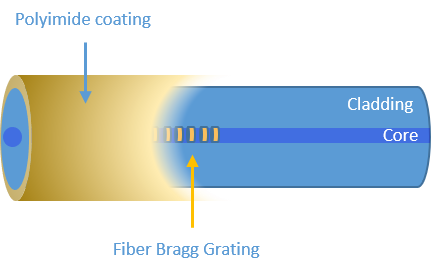
\includegraphics[width=0.45\columnwidth]{Chapter5/images/Picture1.png}
\caption{FBG-based sensors for the RH measurements.}
\label{fig:fbg_scheme}
\end{figure}


It's possible to measure RH instead of strain by applying a hygroscopic material (for example, polyimide or di-ureasil) to the fiber cladding\footnote{Cladding is a layer of material with a lower refractive index that covers the core of a fiber optic cable. The core of the fiber optic cable is of a higher refractive index than the surrounding cladding.} (see figure~\ref{fig:fbg_scheme}). The Bragg wavelength shift becomes the superposition of temperature and humidity effects (see equation~\ref{eqn:FBG})~\cite{Kronenberg:02, YEO_PI}. 
                            %\newpage
                             \begin{equation}\label{eqn:FBG}
                            %\large
                                    \frac{\Delta\lambda_{B}}{\lambda_{B}}=\Delta TS_{T}+\Delta RHS_{RH}
                            \end{equation}
                            where $\lambda_{B}$ is the Bragg wavelength, and $S_{RH/T}$ are the sensitivity coefficients for RH and temperature, respectively. 

Similarly to the strain measurement, it’s crucial to have precise temperature readouts in the vicinity of the coated \gls{FBG}. Otherwise, the actual RH readout may be dominated by uncertainty or just the inaccurate temperature measurement. \gls{FBG} sensors should also be packaged appropriately and kept strain-free to prevent additional stress. Detailed discussion about the experimental setup, chosen design of the \gls{FBG} sensors, and their features will be presented in Section~\ref{fbg_results}.



\subsection{Trace humidity sensing}

Due to expected very low dew point levels inside the \gls{STS} (below \SI{-45}{\celsius}) and the requirement to keep the device safe, it was proposed to use trace humidity sensors in so-called sniffing (sampling) system~\cite{Berruti}. The most common sensing techniques include:
\begin{itemize}
    \item tunable diode laser (dew points from \SI{-100}{\celsius} to \SI{20}{\celsius}),
    \item oscillating quartz crystal sensor (dew points from \SI{-100}{\celsius} to \SI{0}{\celsius}),
    \item aluminum oxide sensor (dew points from \SI{-100}{\celsius} to \SI{20}{\celsius}),
    \item chilled mirror dew point hygrometer  (dew points from \SI{-100}{\celsius} to \SI{100}{\celsius}).
\end{itemize}

Aluminum oxide interacts with water, and it is considered the sensor's sensing layer. In its design, the sensors resemble the capacitive ones. Aluminum oxide based sensors are characterized by very low uncertainties. In addition to that, the implementation in a hardware-based interlock is much easier than in the case of the \gls{FOS} (the readout system is based on analog signals). An example of a sampling system is presented in Figure~\ref{fig:sniffer}. The readout can be placed in distant areas without extensive ionizing radiation or magnetic field. The air is sucked from the detector by a vacuum pump, transported to the sampling cabinet, and then the dew point is measured by the aluminum oxide sensor.  

Another precise and commonly used method, especially for calibration of other humidity sensors, is the chilled mirror hygrometer. The mirror is cooled slowly and in a controlled manner until condensate can be detected on it. Using a vapor pressure curve, it's possible to determine the partial pressure of water vapor at the dew point of flowing gas. A careful measurement presupposes that equilibrium conditions are reached. This can only be achieved by approaching the dew point approximately with the temperature regime and repeating it several times. The measurement range of the Michell S8000 chilled mirror is presented in Figure~\ref{fig:fos_mirror}. The chilled mirror together with the HYT221 and SHT85 were used to calibrate and characterize FBG-based \gls{FOS}. 



\begin{figure}[!h]
\centering
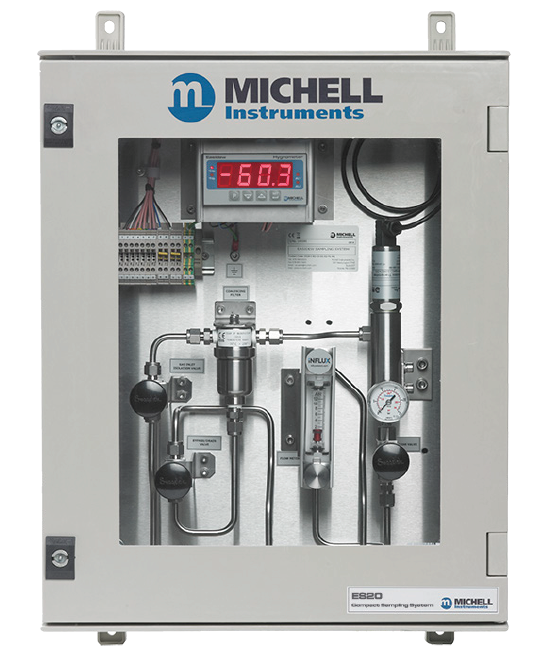
\includegraphics[width=0.35\columnwidth]{Chapter5/images/ES20.png}
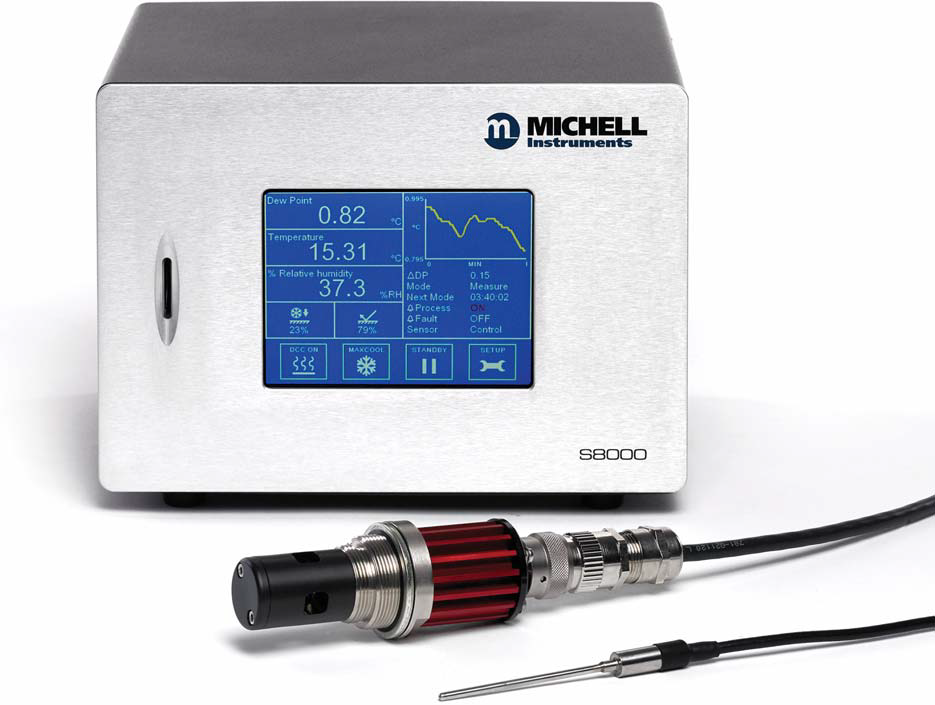
\includegraphics[width=0.4\columnwidth]{Chapter5/images/s8000.png}
\caption{Left: Michell ES20 ceramic metal-oxide sampling system~\cite{michell_e20}
Right: Michell S8000 Remote High Precision Chilled Mirror Hygrometer~\cite{michell_s8000}.}
\label{fig:sniffer}
\end{figure}


\begin{figure}[!h]
\centering
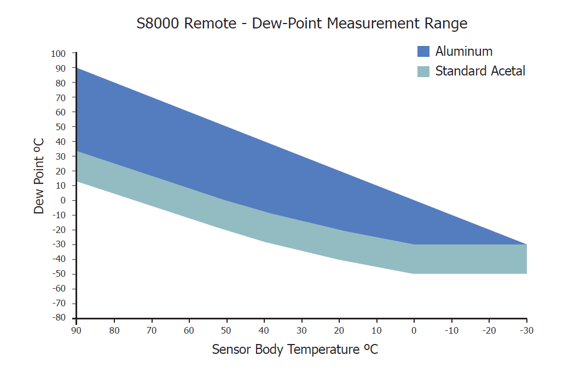
\includegraphics[width=0.65\columnwidth]{Chapter5/images/s8000_remote.png}
\caption{Dew point measuring ranges of S8000 device for two different mirrors~\cite{michell_s8000}.}
\label{fig:fos_mirror}
\end{figure}
\newpage
\subsection{Sensors performance in high radiation environments}
\label{fos_irrad}
Implementing a cost-effective distributed sensing system in highly irradiated environments is a challenging task. Sampling system with multiple sensing lines are considered to be the most reliable way, but their cost per sensing point is relatively high. 

Over the years, capacitive sensors have been widely used in many industrial applications, but their susceptibility to radiation doesn't qualify them as appropriate and reliable sensors for long-term \gls{STS} operation~\cite{Kapic, capacitive_irrad, Berruti}. The sensor's internal electronic circuit is its most vulnerable part~\cite{SHCHEMEROV20222871}.

In recent decades, researchers have studied the effects of different types of radiation on optical fibers. When radiation interacts with materials, it changes their characteristics and often affects the performance and reliability of the devices, with pronounced consequences. For all these reasons, careful investigations concerning how radiation affects the operation of components intended for use in these harsh environments were conducted. The radiation may cause point defects inside the fiber, causing the attenuation of the signal~\cite{FOS_FIB_RAD}. Nowadays, it's possible to fabricate radiation hard fibers \cite{troska}, for example as reported by Berruti~\cite{Berruti} commonly used Corning SMF-28 optical fibers are considered radiation tolerant. However, a careful choice of fiber material is needed, as its reliability depends on many factors such as dose, dose rate, and wavelength.  

A second element that might be sensitive to radiation is the  Fiber Bragg Grating, as the radiation may affect the wavelength shift~\cite{gusarov}. The grating itself can survive high doses, but it's not completely insensitive to the radiation. Similarly, as with the fibers' materials, many factors can influence the response to the radiation of the grating. Some of them like the doping concentration (fiber is often doped with e.g. germanium), or hydrogen loading\footnote{hydrogen is used to increase the sensitivity of the optical fiber to the UV-light laser}~\cite{gusarov}. The next section will clarify the process of choosing the humidity sensor in more detail. 


